\documentclass[a4paper, 12pt]{article}
\usepackage[utf8x]{inputenc}
\usepackage[english, russian]{babel}
\usepackage[left=25mm, top=25mm, right=25mm, bottom=25mm]{geometry}
\usepackage{cmap}
\usepackage{indentfirst}
\usepackage{tikz}
\usepackage{float}
\usepackage{amsmath, amsfonts, amssymb}
\usepackage{graphicx}
\usepackage{hyperref}
\usepackage{listings}
\usepackage{caption}
\usepackage{subcaption}
\usepackage{xcolor}
\usepackage{etoolbox}
\usepackage{titlesec}
\pagestyle{plain}
\patchcmd{\tableofcontents}{\contentsname}{\centering\contentsname}{}{}
\titleformat{\section}[block]{\normalfont\large\bfseries\centering}{}{0pt}{}
\titleformat{\subsection}[block]{\normalfont\normalsize\bfseries\centering}{}{0pt}{}
\allowdisplaybreaks
\graphicspath{{src/images/}}
\usetikzlibrary{patterns}
\definecolor{LightGray}{gray}{0.95}
\definecolor{LightGray2}{gray}{0.7}
\lstdefinestyle{code}{
    language=MATLAB, % replace language here
    basicstyle=\footnotesize\ttfamily,
    % numbers=left,
    % numberstyle=\scriptsize\color{gray},
    % stepnumber=1,
    % numbersep=5pt,
    backgroundcolor=\color{LightGray},
    showspaces=false,
    showstringspaces=false,
    showtabs=false,
    tabsize=4,
    captionpos=b,
    breaklines=true,
    breakatwhitespace=false,
    frame=single,
    rulecolor=\color{LightGray2},
    linewidth=\linewidth,
    keywordstyle=\color{blue}\bfseries,
    commentstyle=\color{green!40!black},
    stringstyle=\color{purple},
    escapeinside={\%*}{*)},
    inputencoding=utf8x,
    xleftmargin=0pt,
    framexleftmargin=0pt,
    framexrightmargin=0pt
}
\lstset{style=code}
\hypersetup{
    colorlinks=true,
    linkcolor=blue,
    filecolor=magenta,
    urlcolor=cyan,
    pdftitle={contents setup},
    pdfpagemode=FullScreen,
}


\begin{document}
    \begin{titlepage}

        \begin{center}
        Федеральное государственное автономное образовательное учреждение высшего образования
        «Национальный Исследовательский Университет ИТМО»
        \vfill
        
        
\includegraphics[width=0.3\textwidth]{itmo.png} % requires /src/images/itmo.png

        {\large\bf ЛАБОРАТОРНАЯ РАБОТА №4}\\
        {\large\bf ПРЕДМЕТ «ТЕОРИЯ АВТОМАТИЧЕСКОГО УПРАВЛЕНИЯ»}\\
        {\large\bf ТЕМА «СЛЕЖЕНИЕ И КОМПЕНСАЦИЯ: ВИРТУАЛЬНЫЙ ВЫХОД»}\\
        Вариант №2
        \vfill

        \begin{flushright}
            \begin{minipage}{.45\textwidth}
            {
                \hbox{Преподаватель:}
                \hbox{Пашенко А. В.}
                \hbox{}
                \hbox{Выполнил:}
                \hbox{Румянцев А. А.}
                \hbox{}
                \hbox{Факультет: СУиР}
                \hbox{Группа: R3341}
                \hbox{Поток: ТАУ R22 бак 1.1.1}
            }
            \end{minipage}
        \end{flushright}
        \vfill
  
        Санкт-Петербург\\
        2025
        \end{center}
    \end{titlepage}
    
    \tableofcontents

    \newpage
    \section{Задание 1. Компенсирующий регулятор по состоянию}
    Рассмотрим систему
    $$
    \dot{x}=Ax+Bu+B_f\omega_f,
    $$
    $$
    A=\begin{bmatrix}
        5 &2 &7\\
        2 &1 &2\\
        -2 &-3 &-4
    \end{bmatrix},\ B=\begin{bmatrix}
        3\\1\\-1
    \end{bmatrix},\ B_f=\begin{bmatrix}
        -4 &0 &0 &-1\\
        0 &0 &0 &0\\
        4 &0 &0 &0
    \end{bmatrix},\ x(0)=\begin{bmatrix}
        0\\0\\0
    \end{bmatrix},
    $$
    генератор внешнего возмущения
    $$
    \dot{\omega}_f=\Gamma\omega_f,\ \Gamma=\begin{bmatrix}
        25 &6 &-20 &11\\
        14 &3 &-10 &4\\
        40 &11 &-31 &17\\
        6 &4 &-4 &3
    \end{bmatrix},\ \omega_f(0)=\begin{bmatrix}
        1\\1\\1\\1
    \end{bmatrix}
    $$
    и виртуальный выход вида
    $$
    z=C_Zx,\ C_Z=\begin{bmatrix}
        -2 &1 &-1
    \end{bmatrix};
    $$

    
    \subsection{Характер внешнего возмущения}
    Для определения характера внешнего возмущения найдем собственные числа матрицы $\Gamma$.
    Программа в \texttt{MATLAB} находится на листинге \ref{task1} в приложении 1
    $$
    \sigma\left( \Gamma \right)=\left\{ \pm i, \pm 3i \right\}
    $$
    Так как спектр состоит только из мнимых собственных чисел, то характер возмущения -- гармоники
    без затухания и роста амплитуды с течением времени.


    \subsection{Схема моделирования системы, замкнутой компенсирующим регулятором}
    Построим схему моделирования системы, замкнутой компенсирующим регулятором
    $$u=K_1x+K_2\omega_f,$$ обеспечивающим выполнение целевого условия $$\lim\limits_{t\to\infty}z(t)=0$$
    при внешнем воздействии, задаваемом генератором. Снимаем осциллограммы $u(t)$, $w_f(t)$, $x(t)$, $z(t)$
    \begin{figure}[H]
        \centering
        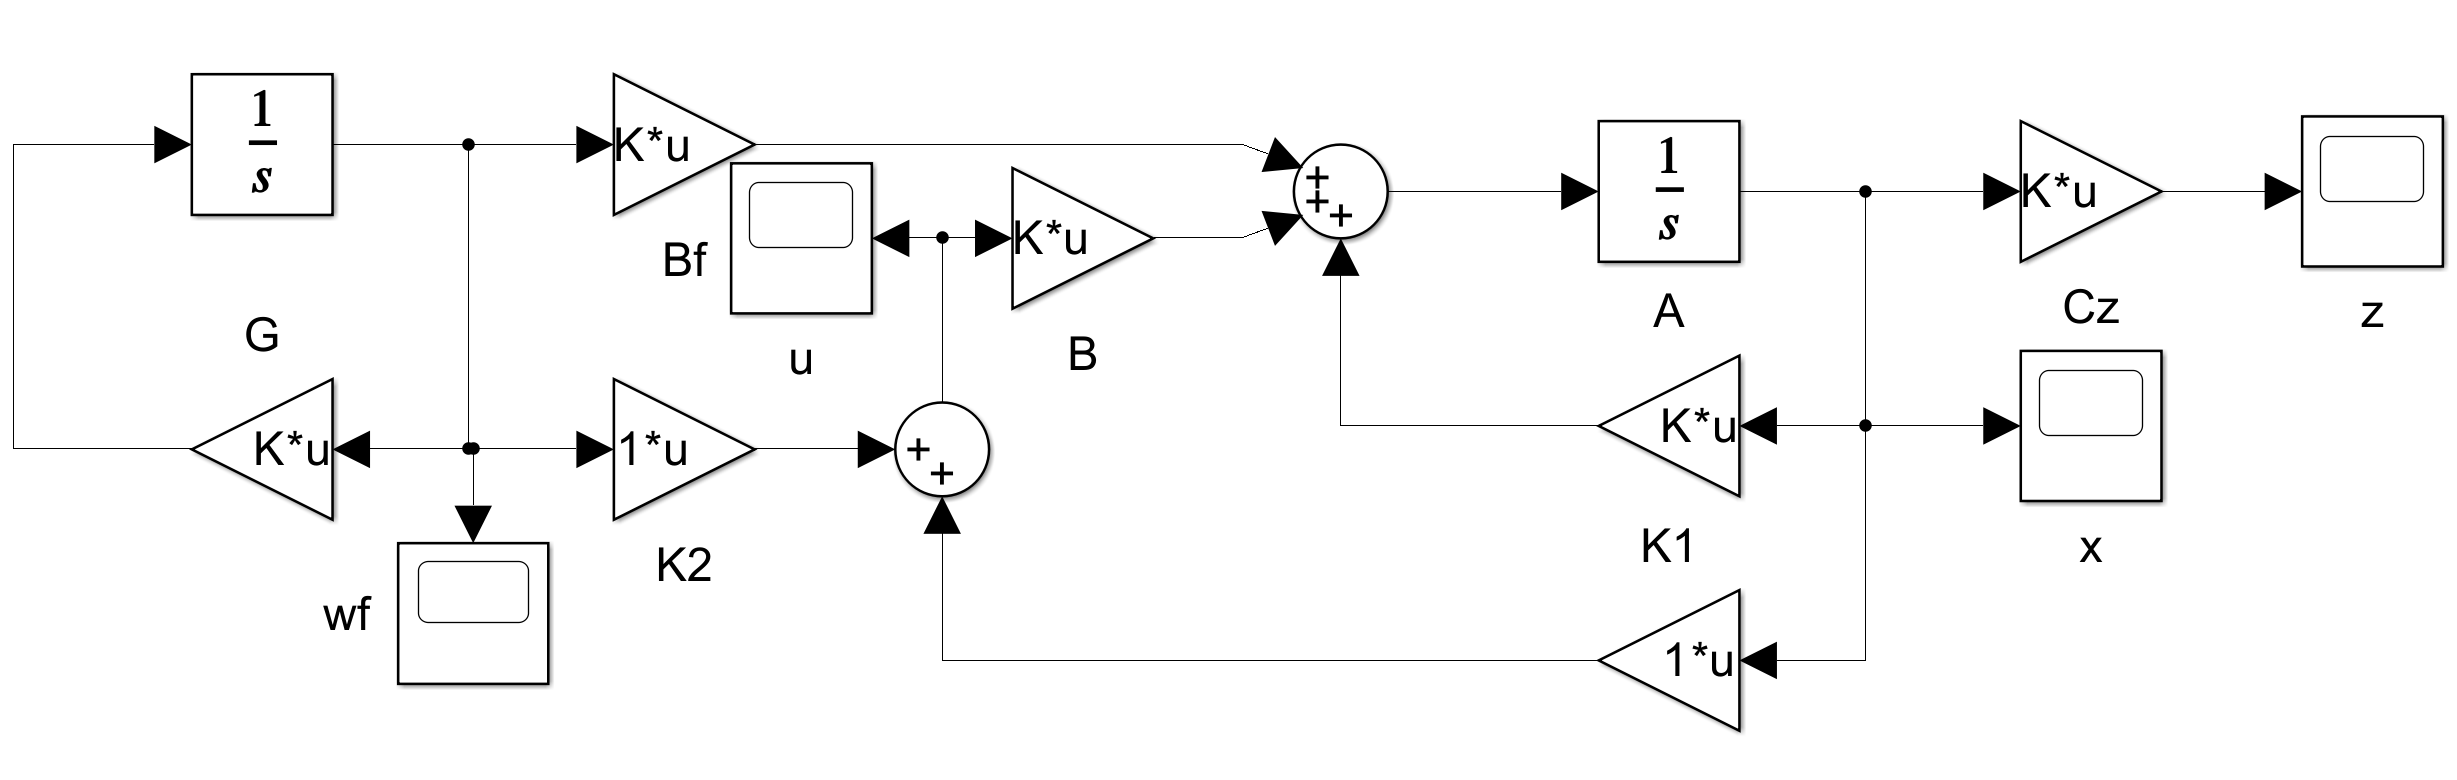
\includegraphics[scale=0.225]{1task_scheme.png}
        \captionsetup{skip=0pt}
        \caption{Схема моделирования системы, замкнутой компенсирующим регулятором}
        \label{fig:1task_scheme}
    \end{figure}


    \subsection{Исследование системы перед синтезом регулятора}
    Определим управляемость и стабилизируемость системы.
    Найдем собственные числа матрицы $A$
    $$
    \sigma\left( A \right)=\left\{ -2,2\pm i \right\}
    $$
    Собственное число $\lambda_1=-2$ асимптотически устойчивое, остальные неустойчивые.
    Выполним жорданово разложение матрицы $A$ в вещественной форме. Найдем вектор
    $B$ в базисе собственных векторов матрицы $A$. Получаем
    $$
    A_{J_{re}}=\begin{bmatrix}
    -2     &0     &0\\
    0     &2     &1\\
    0    &-1     &2
    \end{bmatrix},\ B_{J_{re}}=\begin{bmatrix}
    0\\
     3\\
    -1
    \end{bmatrix};
    $$
    Собственное число $\lambda_1=-2$ неуправляемое, остальные управляемые. Система не полностью управляема,
    стабилизируема. Максимальная степень устойчивости
    $\alpha=|\min{\left(\text{Re}\left( \tilde{\sigma}\left( A \right):\lambda_i\in\mathbb{C}_{-} \right)\right)}|=2$.


    \subsection{Синтез компоненты обратной связи компенсирующего регулятора}
    Синтезируем $K_1$ с помощью матричного уравнения типа Риккати. Зададим
    $Q=0,\ \nu=2,\ R=1$. Решаем при $\alpha=2$. Получаем матрицу регулятора
    $$
    K_1=\begin{bmatrix}
    1.6000  &-11.2000    &1.6000
    \end{bmatrix}
    $$
    Проверим собственные числа замкнутой системы $A+BK_1$
    $$
    \sigma\left( A+BK_1 \right)=\left\{ -2,-2.0000 \pm 4.1231i \right\}
    $$
    Желаемая степень устойчивости достигнута, регулятор синтезирован корректно.


    \subsection{Синтез компоненты прямой связи компенсирующего регулятора}
    Чтобы синтезировать $K_2$, нужно найти $K_1$ (уже нашли), найти $P,Y$
    как решение системы уравнений
    $$
    \begin{cases}
        P\Gamma-AP=BY+B_f\\
        C_ZP+D=0
    \end{cases}
    $$
    и вычислить $K_2$ по формуле
    $$
    K_2=Y-K_1P
    $$
    Предоставим вычисления пакету \texttt{cvx} в \texttt{MATLAB}. Получаем
    $$
    K_2=\begin{bmatrix}
        -48.3631  &-13.0092   &35.7538  &-23.4769
    \end{bmatrix}
    $$


    % pos 885,224,768,358
    \subsection{Компьютерное моделирование}
    Выполним компьютерное моделирование разомкнутой системы $\left( u=0 \right)$;
    системы, замкнутой регулятором только с $K_1$ компонентой; системы, замкнутой компенсирующим регулятором.
    Построим графики вектора состояния генератора внешнего возмущения
    $\omega_f(t)$, формируемого регулятором управления $u(t)$, вектора состояния объекта управления
    $x(t)$ и виртуального выхода $z(t)$.
    Результаты представлены на рис. \ref{fig:1task_wf}--\ref{fig:1task_zz}
    \begin{figure}[H]
        \centering
        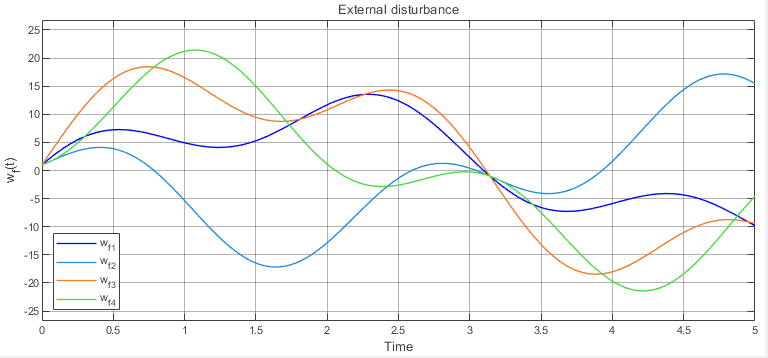
\includegraphics[scale=0.75]{1task_wf.png}
        \captionsetup{skip=0pt}
        \caption{График возмущений $\omega_f(t)$}
        \label{fig:1task_wf}
    \end{figure}
    \begin{figure}[H]
        \centering
        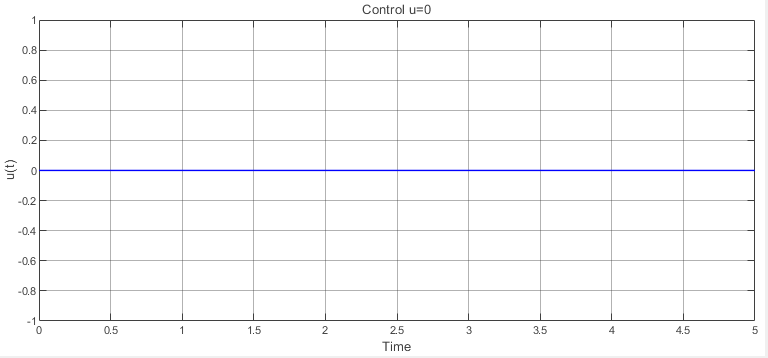
\includegraphics[scale=0.75]{1task_unull_u.png}
        \captionsetup{skip=0pt}
        \caption{График управления $u(t)=0$}
        \label{fig:1task_unull_u}
    \end{figure}
    \begin{figure}[H]
        \centering
        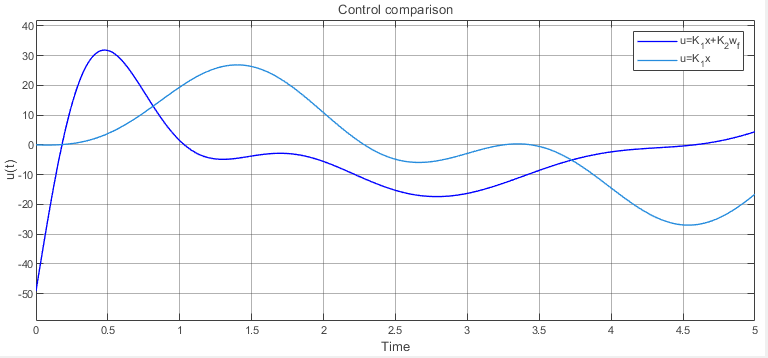
\includegraphics[scale=0.75]{1task_uu.png}
        \captionsetup{skip=0pt}
        \caption{График сравнения управлений $u(t)=K_1x$ и $u(t)=K_1x+K_2\omega_f$}
        \label{fig:1task_uu}
    \end{figure}
    \begin{figure}[H]
        \centering
        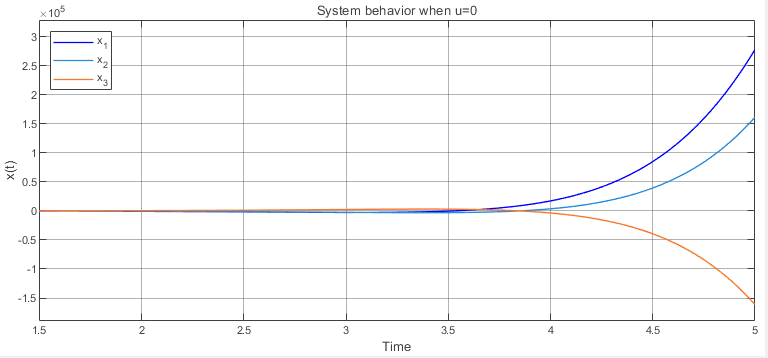
\includegraphics[scale=0.75]{1task_unull_x.png}
        \captionsetup{skip=0pt}
        \caption{График поведения системы $x(t)$ при $u(t)=0$}
        \label{fig:1task_unull_x}
    \end{figure}
    \begin{figure}[H]
        \centering
        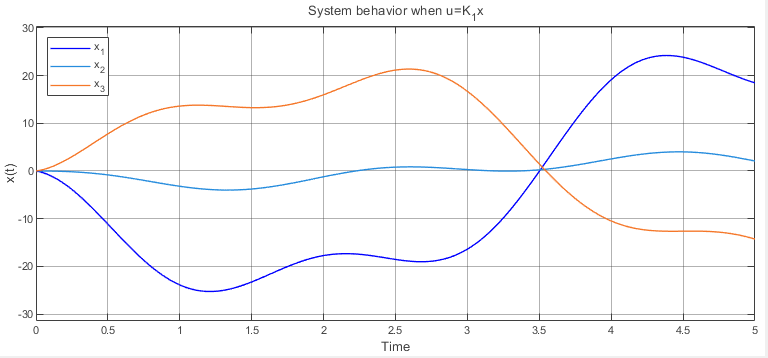
\includegraphics[scale=0.75]{1task_uk_x.png}
        \captionsetup{skip=0pt}
        \caption{График поведения системы $x(t)$ при $u(t)=K_1x$}
        \label{fig:1task_uk_x}
    \end{figure}
    \begin{figure}[H]
        \centering
        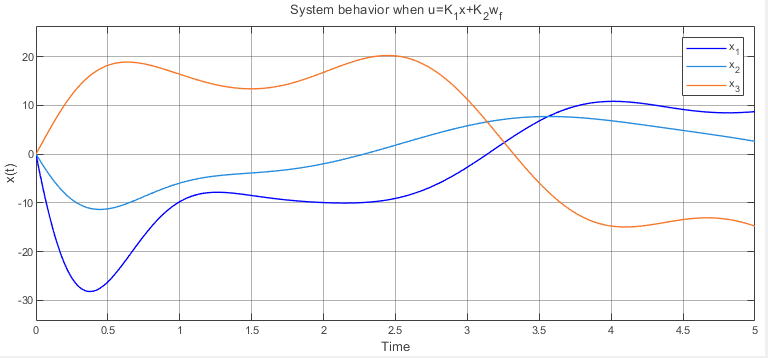
\includegraphics[scale=0.75]{1task_ukk_x.png}
        \captionsetup{skip=0pt}
        \caption{График поведения системы $x(t)$ при $u(t)=K_1x+K_2\omega_f$}
        \label{fig:1task_ukk_x}
    \end{figure}
    \begin{figure}[H]
        \centering
        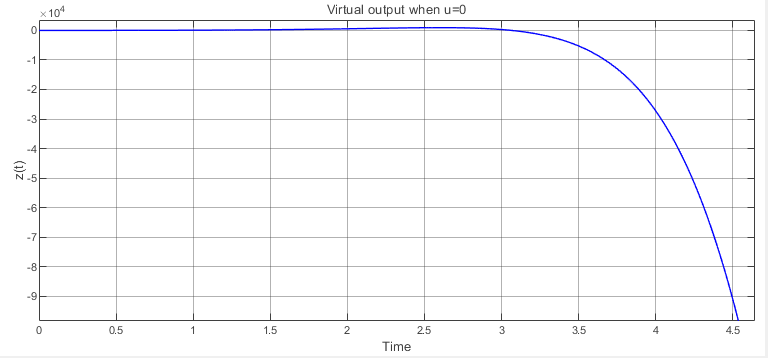
\includegraphics[scale=0.75]{1task_unull_z.png}
        \captionsetup{skip=0pt}
        \caption{График виртуального выхода $z(t)$ при $u(t)=0$}
        \label{fig:1task_unull_z}
    \end{figure}
    \begin{figure}[H]
        \centering
        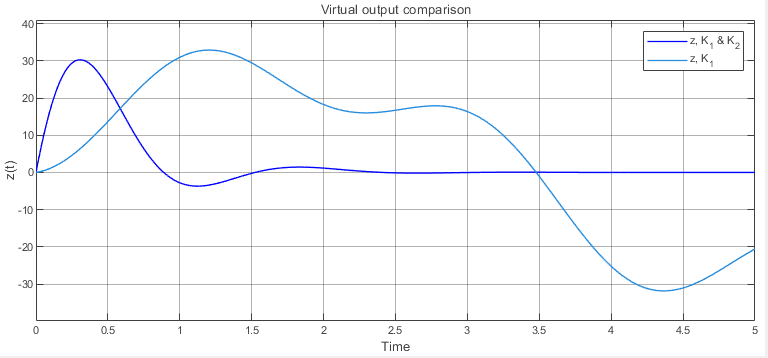
\includegraphics[scale=0.75]{1task_zz.png}
        \captionsetup{skip=0pt}
        \caption{График сравн. виртуальных выходов $z(t)$ при $u(t)=K_1x$ и $u(t)=K_1x+K_2\omega_f$}
        \label{fig:1task_zz}
    \end{figure}
    \noindent Траектория $z(t)$ при компенсирующем регуляторе стремится к нулю -- регулятор выполнил свою задачу.
    При отсутствии $K_2$ компоненты $z(t)$ не стабилизируется, но и не расходится (см. рис. \ref{fig:1task_zz}). При разомкнутой системе
    виртуальный выход расходится (см. рис. \ref{fig:1task_unull_z}). При отсутствии управления вектор
    состояния объекта управления расходится, при наличии -- нет, но и не стабилизируется (см. рис. \ref{fig:1task_unull_x}, \ref{fig:1task_uk_x}, \ref{fig:1task_ukk_x}).
    При наличии $K_2$ компоненты регулятор сразу начинает действовать на объект управления, при наличии только $K_1$ компоненты
    регулятор постепенно управляет системой (см. рис. \ref{fig:1task_uu}).


    \subsection{Вывод}
    В данном задании был исследован компенсирующий регулятор по состоянию.
    Был синтезирован компенсирующий регулятор. Было проведено компьютерное
    моделирование при различных конфигурациях регулятора.
    Результаты были сравнены. Компенсирующий регулятор был синтезирован корректно.


    \section{Задание 2. Следящий регулятор по состоянию}
    Рассмотрим систему (матрицы $A,B,C_Z,\Gamma$ такие же, как в задании 1)
    $$
    \dot{x}=Ax+Bu,\ x(0)=\begin{bmatrix}
        1 &1 &1
    \end{bmatrix}^T,
    $$
    генератор задающего сигнала
    $$
    \dot{\omega}_g=\Gamma\omega_g,\ \omega_g(0)=\begin{bmatrix}
        1 &1 &1 &1
    \end{bmatrix}^T
    $$
    и виртуальный выход вида
    $$
    z=C_Zx+D_Z\omega_g,\ D_Z=\begin{bmatrix}
        -20 &-6 &16 &-9
    \end{bmatrix};
    $$


    \subsection{Характер внешнего возмущения}
    Матрица $\Gamma$ такая же, как в первом задании. Ее спектр имеет вид
    $$
    \sigma\left( \Gamma \right)=\left\{ \pm i, \pm 3i \right\}
    $$
    Характер возмущений -- гармоники без затухания и роста амплитуды с течением времени.


    \subsection{Схема моделирования системы, замкнутой следящим регулятором}
    Построим схему моделирования системы, замкнутой следящим регулятором
    $$
    u=K_1x+K_2\omega_g,
    $$
    обеспечивающим выполнение целевого условия
    $$\lim\limits_{t\to\infty}z(t)=0$$
    при внешнем воздействии, задаваемом генератором. Снимаем осциллограммы $u(t)$, $w_g(t)$, $x(t)$, $z(t)$
    \begin{figure}[H]
        \centering
        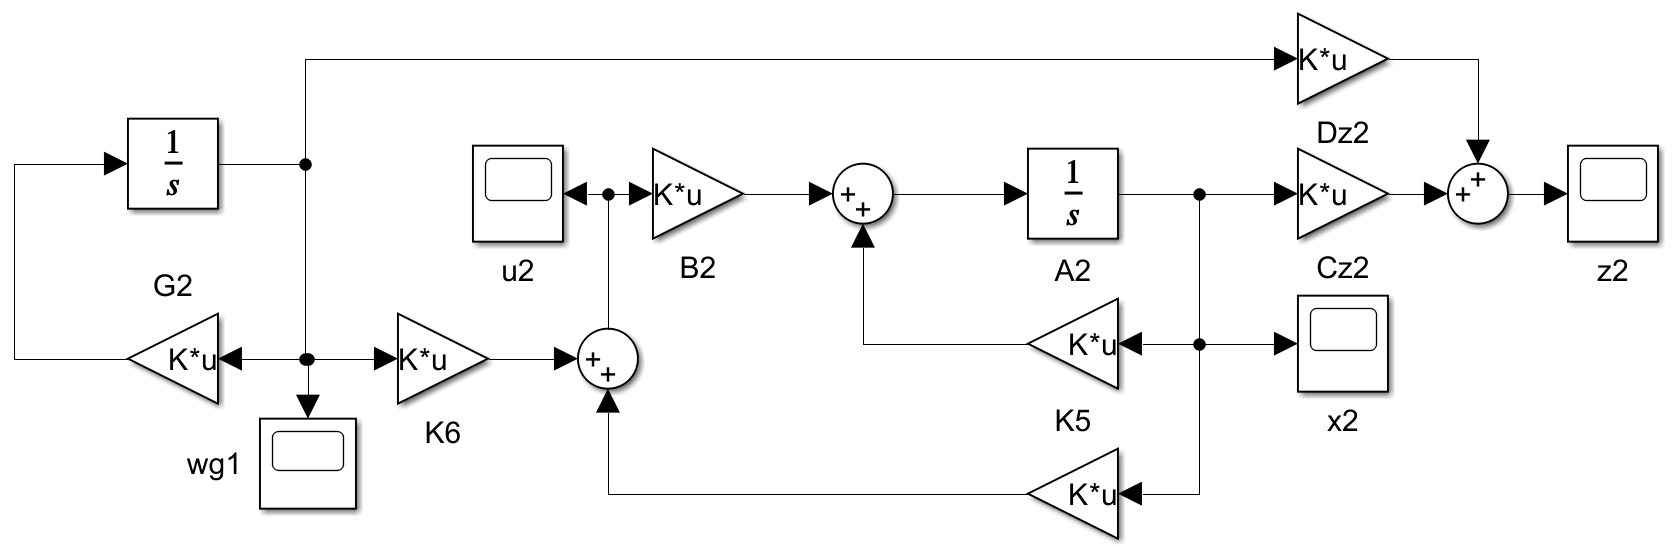
\includegraphics[scale=0.325]{2task_scheme.png}
        \captionsetup{skip=0pt}
        \caption{Схема моделирования системы, замкнутой следящим регулятором}
        \label{fig:2task_scheme}
    \end{figure}


    \subsection{Исследование системы перед синтезом регулятора}
    Матрицы $A,B$ такие же, как в первом задании. Имеем
    $$
    \sigma\left( A \right)=\left\{ -2,2\pm i \right\},\ A_{J_{re}}=\begin{bmatrix}
        -2     &0     &0\\
        0     &2     &1\\
        0    &-1     &2
        \end{bmatrix},\ B_{J_{re}}=\begin{bmatrix}
        0\\
         3\\
        -1
        \end{bmatrix};
    $$
    Система не полностью управляема, стабилизируема. Максимальная степень устойчивости $\alpha=2$.


    \subsection{Синтез компоненты обратной связи следящего регулятора}
    Синтезируем $K_1$ так же, как в задании 1 -- с помощью матричного уравнения Риккати.
    Матрицы, участвующие в расчетах, не изменились. Таким образом, имеем
    $$
    K_1=\begin{bmatrix}
    1.6000  &-11.2000    &1.6000
    \end{bmatrix},\
    \sigma\left( A+BK_1 \right)=\left\{ -2,-2.0000 \pm 4.1231i \right\};
    $$
    В первом задании уже выяснили, что регулятор синтезирован корректно.


    \subsection{Синтез компоненты прямой связи следящего регулятора}
    Синтезируем $K_2$ аналогично заданию 1. Из системы уравнений пропадет $B_f$, взамен появится $D_Z$.
    Программа представлена на листинге \ref{task2} в приложении 2. Получаем
    $$
    K_2=\begin{bmatrix}
        7.2    &3.2  &-8.0  &4.0
    \end{bmatrix}
    $$


    \subsection{Компьютерное моделирование}
    Выполним компьютерное моделирование систем аналогично заданию 1
    \begin{figure}[H]
        \centering
        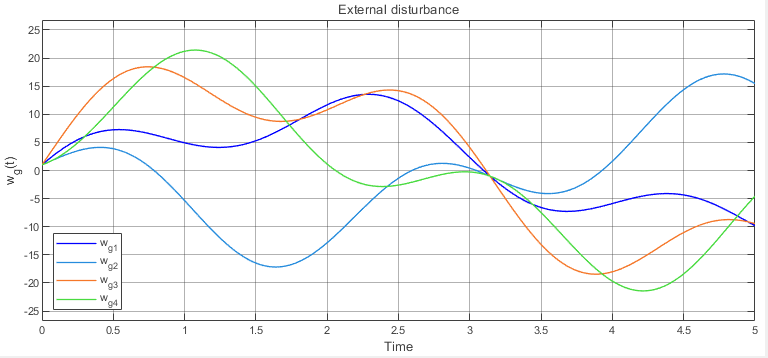
\includegraphics[scale=0.75]{2task_wg.png}
        \captionsetup{skip=0pt}
        \caption{График возмущений $\omega_g(t)$}
        \label{fig:2task_wg}
    \end{figure}
    \begin{figure}[H]
        \centering
        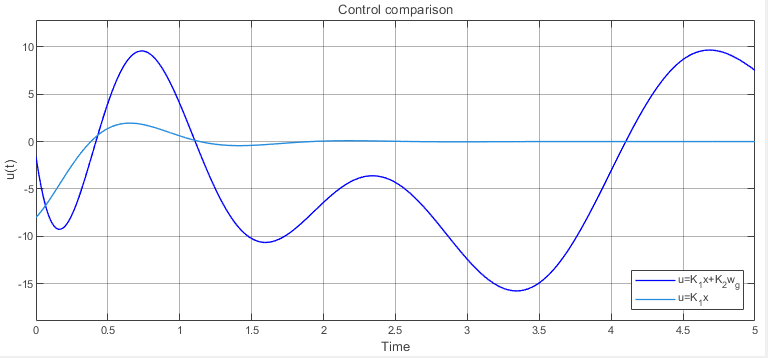
\includegraphics[scale=0.75]{2task_uu.png}
        \captionsetup{skip=0pt}
        \caption{График сравнения управлений $u(t)=K_1x$ и $u(t)=K_1x+K_2\omega_g$}
        \label{fig:2task_uu}
    \end{figure}
    \begin{figure}[H]
        \centering
        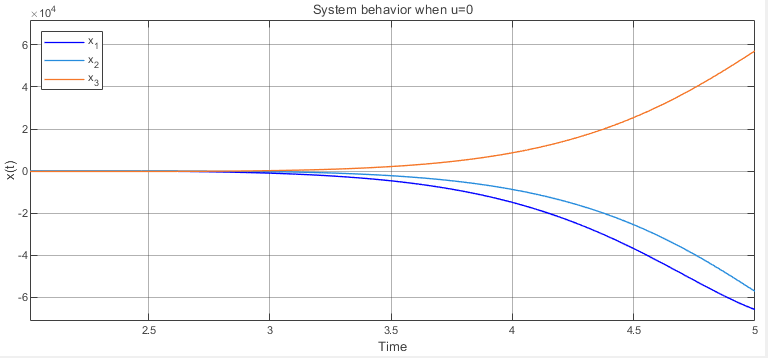
\includegraphics[scale=0.75]{2task_unull_x.png}
        \captionsetup{skip=0pt}
        \caption{График поведения системы $x(t)$ при $u(t)=0$}
        \label{fig:2task_unull_x}
    \end{figure}
    \begin{figure}[H]
        \centering
        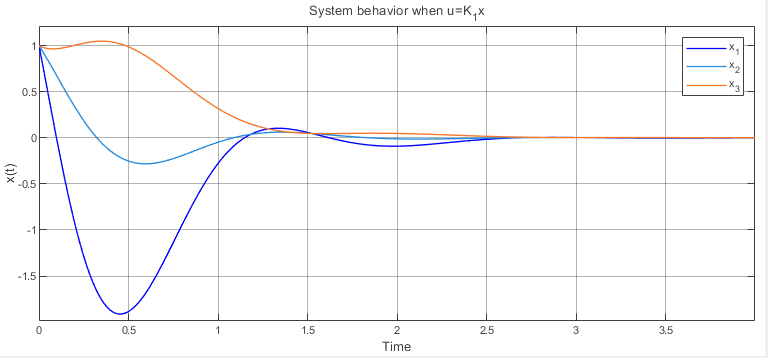
\includegraphics[scale=0.75]{2task_uk_x.png}
        \captionsetup{skip=0pt}
        \caption{График поведения системы $x(t)$ при $u(t)=K_1x$}
        \label{fig:2task_uk_x}
    \end{figure}
    \begin{figure}[H]
        \centering
        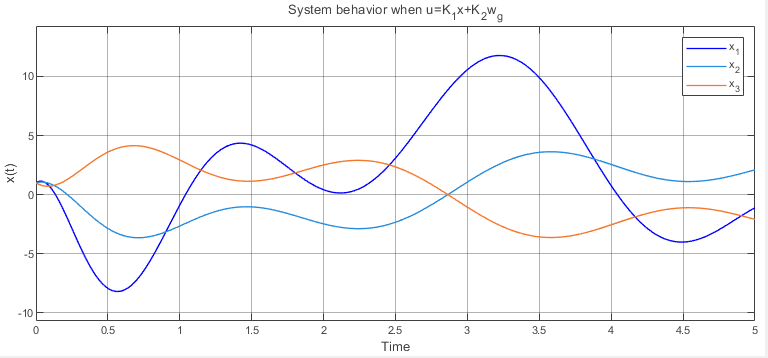
\includegraphics[scale=0.75]{2task_ukk_x.png}
        \captionsetup{skip=0pt}
        \caption{График поведения системы $x(t)$ при $u(t)=K_1x+K_2\omega_g$}
        \label{fig:2task_ukk_x}
    \end{figure}
    \begin{figure}[H]
        \centering
        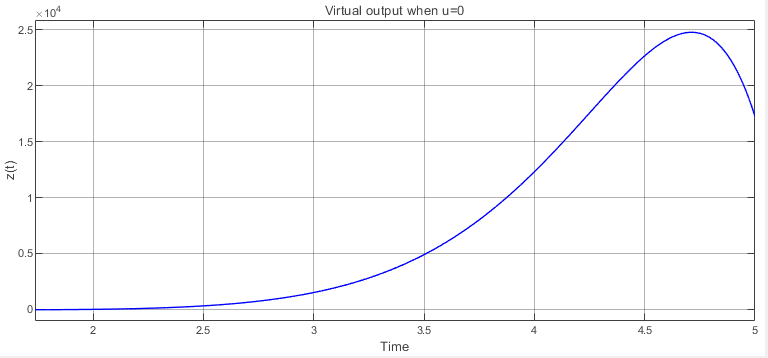
\includegraphics[scale=0.75]{2task_unull_z.png}
        \captionsetup{skip=0pt}
        \caption{График виртуального выхода $z(t)$ при $u(t)=0$}
        \label{fig:2task_unull_z}
    \end{figure}
    \begin{figure}[H]
        \centering
        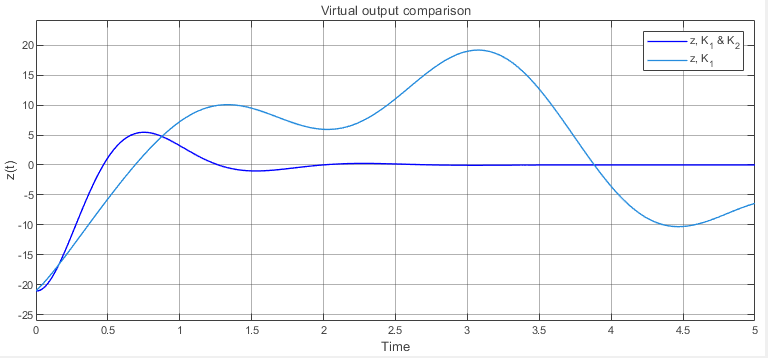
\includegraphics[scale=0.75]{2task_zz.png}
        \captionsetup{skip=0pt}
        \caption{График сравн. виртуальных выходов $z(t)$ при $u(t)=K_1x$ и $u(t)=K_1x+K_2\omega_g$}
        \label{fig:2task_zz}
    \end{figure}
    \noindent Следящий регулятор выполнил свою задачу -- на рис. \ref{fig:2task_zz}
    $z(t)$ стремится к нулю с увеличением времени. Виртуальный выход для регулятора только
    с компонентой $K_1$ не расходится, но и не стабилизируется. При отсутствии управления $z(t)$
    расходится (см. рис. \ref{fig:2task_unull_z}). Вектор состояния объекта управления под действием
    регулятора только с $K_1$ компонентой стабилизируется к нулю, но виртуальный выход продолжает
    движение под действием внешних возмущений ($C_Zx\rightarrow0,D_Z\omega_g\nrightarrow0$).
    При наличии компонент $K_1,K_2$ график $x(t)$ не стабилизируется к нулю, но и не расходится (см. рис. \ref{fig:2task_ukk_x}),
    при этом $z(t)$ достигает целевого состояния. Без управления $x(t)$ расходится (см. рис. \ref{fig:2task_unull_x}).
    При наличии только компоненты $K_1$ управление со временем стабилизируется к нулю, при наличии обеих компонент -- нет (см. рис. \ref{fig:2task_uu}).


    \subsection{Вывод}
    В данном задании был исследован следящий регулятор по состоянию.
    Его синтез был проведен аналогично синтезу компенсирующего регулятора в задании 1.
    Было выполнено компьютерное моделирование систем со сравнением результатов.


    \section{Общий вывод по работе}
    ...


    \section{Приложения}
    \subsection{Приложение 1}
    \begin{lstlisting}[label=task1, caption={Программа для задания 1}]
    % plant parameters
    A = [5 2 7;
         2 1 2;
        -2 -3 -4];
    B = [3; 1; -1];
    Bf = [-4 0 0 -1;
          0 0 0 0;
          4 0 0 0];

    G = [25 6 -20 11;
         14 3 -10 4;
         40 11 -31 17;
         6 4 -4 3];

    Cz = [-2 1 -1];
    D = 0;

    % G eigenvalues
    G_eig = eig(G)

    % A eigenvalues
    A_eig = eig(A)

    % Jordan matrix
    [Aj, J] = jordan(A);
    Pjre(:,1) = Aj(:,1);
    Pjre(:,2) = imag(Aj(:,2));
    Pjre(:,3) = real(Aj(:,3))
    Pjre_inv = Pjre^-1
    Aj_re = Pjre_inv * A * Pjre
    B_jre = Pjre_inv * B

    % solving Riccati
    Q = 0;
    v = 2;
    R = 1;
    a = 2;

    Aa = A + eye(3) * a;
    [Pk,K,e]=icare(Aa,sqrt(2)*B,Q,R);
    K1=-inv(R)*B'*Pk
    eK1=eig(A+B*K1)

    % K2 regulator synthesis
    cvx_begin sdp
    variable P(3,4)
    variable Y(1,4)
    P*G-A*P == B*Y+Bf;
    Cz*P + D == 0;
    cvx_end

    K2 = Y-K1*P
    \end{lstlisting}


    \subsection{Приложение 2}
    \begin{lstlisting}[label=task2, caption={Программа для задания 2}]
    % plant parameters
    A = [5 2 7;
         2 1 2;
        -2 -3 -4];
    B = [3; 1; -1];
    Bg = 0;

    G = [25 6 -20 11;
         14 3 -10 4;
         40 11 -31 17;
         6 4 -4 3];

    Cz = [-2 1 -1];
    Dz = [-20 -6 16 -9];

    % solving Riccati
    Q = 0;
    v = 2;
    R = 1;
    a = 2;

    Aa = A + eye(3) * a;
    [Pk,K,e]=icare(Aa,sqrt(2)*B,Q,R);
    K1=-inv(R)*B'*Pk
    eK1=eig(A+B*K1)

    % K2 regulator synthesis
    cvx_begin sdp
    variable P(3,4)
    variable Y(1,4)
    P*G-A*P == B*Y+Bg;
    Cz*P + Dz == 0;
    cvx_end

    K2 = Y-K1*P
    \end{lstlisting}
\end{document}